\documentclass[12pt,a4paper,oneside]{article} %% Dokumenten Parameter und Art des Dokuments
\usepackage[utf8x]{inputenc} %% Diese Datei ist im utf8 Format dies ist hier damit Latex uns versteht
\usepackage[ngerman]{babel} %% Rechtschreib prüfung
\usepackage{hyperref}
\usepackage{amsmath} %% Packet zur verwendung Mathematischer Formeln
\usepackage{amsfonts}
\usepackage{amssymb} %% Packet zur verwendung Mathematischer Symbole
\usepackage{mathtools}
\usepackage{microtype} %% Sorgt für besseren umgang mit zu lange/kurzen Zeilen
\usepackage{pdfpages} %% Zum einfügen eines PDf dokuments
\title{TGI Serie 8}
\author{Bennet Bleßmann, Sven Korfmann}

\begin{document}
\maketitle

\section*{H1}


\section*{H2}
Beweis über Induktion: \\
IA:
n=0\\
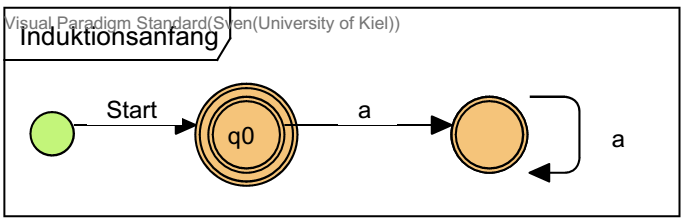
\includegraphics[scale=1]{part/TGIS08A02} \\
Ist minimal da Mindesten eine Entscheidung getroffen werden muss, ein akzeptierender und ein verwerfender Zustand.\\
\\
IS: \\
Nehme $n \in N$ dann nehme $|Q_{n-1}|$ minimal (IH) für n-1 nun muss mindestenz 1 Zustand hinzugefügt werden um $Q_n$ zu prüfen, damit ist $|Q_n|>n-1 \Leftrightarrow |Q_n| \geq n$

\section*{H3}
Sei M TM wie folgt:\\
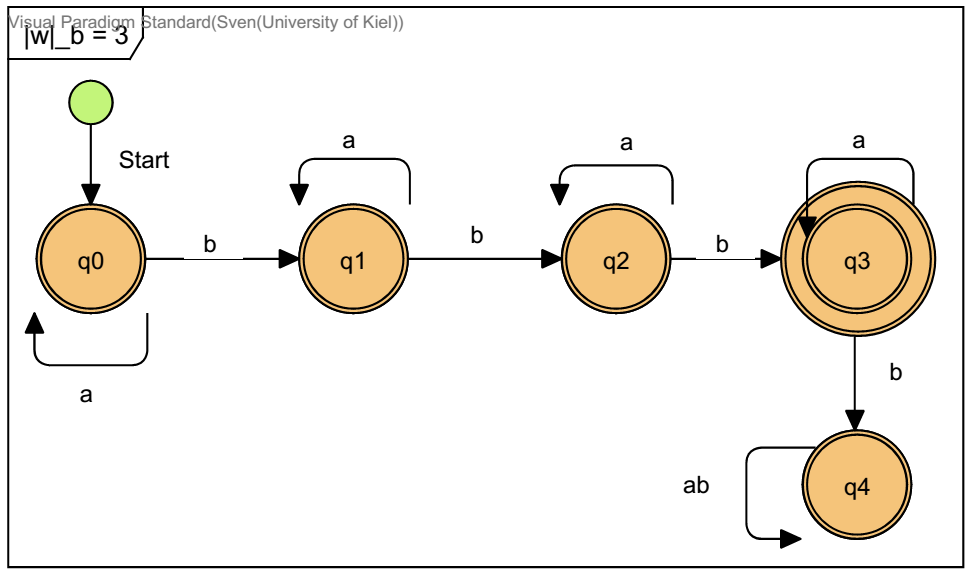
\includegraphics[scale=0.8]{part/TGIS08A03}
Beweis dass  $L(M)=L$:\\
Seien $u,v,x,y$ $\in a^* $ und $t \in \Sigma^*$\\
$\hat{\delta}(q_0,ubv)= \hat{\delta}(\delta (\hat{ \delta} (q_0,v),b), u) = \hat{\delta}(\delta (q_0,b), u) = \hat{\delta}(q_1, u) = q_1$ was nicht akzeptierend ist und $|ubv|_b=1$ $ubv\notin L$\\
\\
$\hat{\delta}(q_0,ubvbx)=\hat{\delta} ( \delta( \hat{\delta}(\delta (\hat{ \delta} (q_0,u),b), v),b),x) =\hat{\delta} ( \delta( \hat{\delta}(\delta (q_0,b), v),b),x) =\hat{\delta} ( \delta( \hat{\delta}(q_1, v),b),x) = \hat{\delta} ( \delta( q_1,b),x) = \hat{\delta} ( q_2),x) = q_2 $ was nicht akzeptierend ist und $|ubvbx|_b=2$ $ubvbx\notin L$\\
\\
$\hat{\delta}(q_0,ubvbxby)=\hat{\delta} ( \delta(\hat{ \delta} (q_0,ubvbx),b),y) = \hat{\delta}(\delta ( q_2),b),y) =\hat{\delta}(q_3,y)= q_3 $ was akzeptierend ist und $|ubvbxby|_b=3$ $ubvbxby\in L$\\
\\
$\hat{\delta}(q_0,ubvbxbybt)=\hat{\delta}(\delta ( \hat{\delta}(q_0,ubvbxby),b),t)=\hat{\delta}(\delta (q_3,b),t)=\hat{\delta}(q_4,t) = q_4  $ was nicht akzeptierend ist und $|ubvbxbybt|_b>3$ $ubvbxbybt\notin L$\\
\\
Somit sind alle $|w|_b$ Fälle abgedeckt und nur $|w|_b=3$ wird von M akzeptiert somit gilt $L(M)=L$



\section*{H4}

\subsection*{1)}

Die Aussage in Worten: Es gibt keine Transition zum Startzustand.
$N$ erweitern wir nun um einen neuen Startzustand $q_{0M}$ und entsprechende Transitionen zu $M_1$.

$q_{0_N} \in F_N \Leftrightarrow q_{0_{M_i}} \in F_{M_1}$ 

$F_N  =  F_{M_1} \setminus \{q_{0_{M_i}}\}$

$Q_{M_1} = Q_N \cup \{q_{0_{M_i}}\}$

$\forall q \in Q_{M_1}, a \in \Sigma: \delta_{M_1}(q,a) = 
\begin{cases}
\delta_N(q,a) \textit{ , für }q \neq q_{0_{M_1}} \\
\delta_N(q_{0_N},a) \textit{ , für }q = q_{0_{M_1}}
\end{cases}$ 

\subsection*{2)}

Die Aussage in Worten: Alle Zustände für die eine ausgehende Transition existiert sind nicht akzeptierende Zustände.

Da bei DEA's für jeden Zustand und jedes Eingabe Symbol ein Folge Zustand durch $\delta_{M_2}$ definiert sein muss existiert immer eine  ausgehende Transition, somit darf kein Zustand Endzustand sein d.h. $M_1$ kann nur für $L(N) = \varnothing$  definiert werden als ein Automaten mit einem nicht akzeptierendem Zustand und einem Self-Loop für alle Eingabesymbole.


\subsection*{3)}

Die Aussage in Worten: Wenn zwei Transitionen zum selben Zustand führen dann waren die Eingabesymbole identisch.

Wir erstellen für jedes Eingabesymbol eine Kopie jedes Zustandes.

$Q_{M_3} = \{q_{(q_N,a)}|q_N \in Q_N \wedge a \in \Sigma \}$

Wähle einen der Zustände mit $q_{0_N}$ im Index als Startzustand.

$q_{0_{M_3}} \in \{q(q_{0_N},a) \in Q_{M_3}| a \in \Sigma \}$

$\forall q_{(q_N,a_q)} \in Q_{M_3}, a \in \Sigma: 
\delta_{M_3}((q_N,a_q),a) = q_{(\delta_N(q_N,a),a)} $


$F_{M_3} = \{q_{(q_N,a)} \in Q_{M_3} | q_N \in F_N\}$

\subsection*{4)}

Die Aussage in Worten: Wenn ein Zustand q zwei Transitionen (dürfen auch identisch sein) besitzt sind die Eingabesymbole der Transitionen gleich.

Da für jeden Zustand und jedes Eingabesymbol beim DEA eine Transition definiert sein muss ist für $|\Sigma|>1$ die Aussage immer Falsch und für $|\Sigma| = 1$ immer Wahr.
\section*{H5}

\subsection*{2)}

Jeder akzeptierenden Zustände wird nicht akzeptierend und erhält eine $\varepsilon$ 
Transition zu einem neuen akzeptierendem Zustand ohne ausgehende Transitionen.

$Q_{M_2} = Q_N \cup \{q_F\}$

$q_{0_{M_2}} = q_{0_N}$

$\forall q \in Q_{M_2}, a \in \Sigma \cup \{\varepsilon\}:
\delta_{M_2}(q,a) =
\begin{cases}
\varnothing \textit{ , für }q = q_F \\
\varnothing \textit{ , für }q \notin F_N \wedge a = \varepsilon \\
\{\delta_N(q,a)\} \textit{ , für } q \neq q_F \wedge a \neq \varepsilon \\
\{q_F\} \textit{ , für } q \in F_N \wedge a = \varepsilon
\
\end{cases}$

$F_{M_2} = \{q_F\}$

\subsection*{4)}

Wir kopieren die Zustände wie bei M_3 wobei jeder Zustand nur eine nicht Epsilon Transition hat für das Symbol welches der Zustand im Index hat, zwischen den Zuständen mit dem gleichen Zustand im Index existieren Epsilon transitionen.
	
\end{document}